\documentclass[12pt, titlepage]{article}

\usepackage{fullpage}
\usepackage[round]{natbib}
\usepackage{multirow}
\usepackage{booktabs}
\usepackage{tabularx}
\usepackage{array}
\usepackage{longtable}
\usepackage{graphicx}
\usepackage{float}
\usepackage{caption}
\usepackage{tikz}
\usetikzlibrary{arrows.meta, positioning}
\usepackage{hyperref}
\hypersetup{
    colorlinks,
    citecolor=blue,
    filecolor=black,
    linkcolor=red,
    urlcolor=blue
}

\input{../../Comments}
%% Common Parts

\newcommand{\progname}{Software Engineering} % PUT YOUR PROGRAM NAME HERE
\newcommand{\authname}{Team \#5, Money Making Mauraders
\\ Zhenia Sigayev
\\ Justin Ho
\\ Thomas Wang
\\ Michael Shi
\\ Johnny Qu
}


\usepackage{hyperref}
    \hypersetup{colorlinks=true, linkcolor=blue, citecolor=blue, filecolor=blue,
                urlcolor=blue, unicode=false}
    \urlstyle{same}
                                


\newcounter{acnum}
\newcommand{\actheacnum}{AC\theacnum}
\newcommand{\acref}[1]{AC\ref{#1}}

\newcounter{ucnum}
\newcommand{\uctheucnum}{UC\theucnum}
\newcommand{\uref}[1]{UC\ref{#1}}

\newcounter{mnum}
\newcommand{\mthemnum}{M\themnum}
\newcommand{\mref}[1]{M\ref{#1}}
\newcolumntype{L}[1]{>{\raggedright\arraybackslash}p{#1}}
\setlength{\LTcapwidth}{\textwidth}
\captionsetup[longtable]{justification=raggedright,singlelinecheck=false}

\begin{document}

\title{Module Guide for \progname{}} 
\author{\authname}
\date{\today}

\maketitle

\pagenumbering{roman}

\section{Revision History}

\begin{tabularx}{\textwidth}{p{3cm}p{2cm}X}
\toprule {\bf Date} & {\bf Version} & {\bf Notes}\\
\midrule
Wednesday, January 14, 2026 & 1.2 & Added longtable pagination and uses diagram.\\
Monday, November 11, 2025 & 1.1 & Implemented traceability pagination and new uses diagram proof of concept.\\
\bottomrule
\end{tabularx}

\newpage

\section{Reference Material}

This section records information for easy reference.

\subsection{Abbreviations and Acronyms}

\renewcommand{\arraystretch}{1.2}
\begin{tabular}{l l} 
  \toprule		
  \textbf{symbol} & \textbf{description}\\
  \midrule 
  AC & Anticipated Change\\
  API & Application Programming Interface \\
  BUC & Business Use Case \\
  CI/CD & Continuous Integration/Continuous Deployment \\
  DAG & Directed Acyclic Graph \\
  FRQ & Functional Requirement \\
  M & Module \\
  MG & Module Guide \\
  MES & McMaster Engineering Society \\
  OCR & Optical Character Recognition \\
  OS & Operating System \\
  RBAC & Role-Based Access Control \\
  R & Requirement\\
  SRS & Software Requirements Specification\\
  SSO & Single Sign-On \\
  UC & Unlikely Change \\
  UI & User Interface \\
  UX & User Experience \\
  WCAG & Web Content Accessibility Guidelines \\
  \bottomrule
\end{tabular}\\

\newpage

\tableofcontents

\listoftables

\listoffigures

\newpage

\pagenumbering{arabic}

\section{Introduction}

Decomposing a system into modules is a commonly accepted approach to developing
software.  A module is a work assignment for a programmer or programming
team~\citep{ParnasEtAl1984}.  We advocate a decomposition
based on the principle of information hiding~\citep{Parnas1972a}.  This
principle supports design for change, because the ``secrets'' that each module
hides represent likely future changes.  Design for change is valuable in SC,
where modifications are frequent, especially during initial development as the
solution space is explored.  

Our design follows the rules layed out by \citet{ParnasEtAl1984}, as follows:
\begin{itemize}
\item System details that are likely to change independently should be the
  secrets of separate modules.
\item Each data structure is implemented in only one module.
\item Any other program that requires information stored in a module's data
  structures must obtain it by calling access programs belonging to that module.
\end{itemize}

After completing the first stage of the design, the Software Requirements
Specification (SRS), the Module Guide (MG) is developed~\citep{ParnasEtAl1984}. The MG
specifies the modular structure of the system and is intended to allow both
designers and maintainers to easily identify the parts of the software.  The
potential readers of this document are as follows:

\begin{itemize}
\item New project members: This document can be a guide for a new project member
  to easily understand the overall structure and quickly find the
  relevant modules they are searching for.
\item Maintainers: The hierarchical structure of the module guide improves the
  maintainers' understanding when they need to make changes to the system. It is
  important for a maintainer to update the relevant sections of the document
  after changes have been made.
\item Designers: Once the module guide has been written, it can be used to
  check for consistency, feasibility, and flexibility. Designers can verify the
  system in various ways, such as consistency among modules, feasibility of the
  decomposition, and flexibility of the design.
\end{itemize}

The rest of the document is organized as follows. Section
\ref{SecChange} lists the anticipated and unlikely changes of the software
requirements. Section \ref{SecMH} summarizes the module decomposition that
was constructed according to the likely changes. Section \ref{SecConnection}
specifies the connections between the software requirements and the
modules. Section \ref{SecMD} gives a detailed description of the
modules. Section \ref{SecTM} includes two traceability matrices. One checks
the completeness of the design against the requirements provided in the SRS. The
other shows the relation between anticipated changes and the modules. Section
\ref{SecUse} describes the use relation between modules.

\section{Anticipated and Unlikely Changes} \label{SecChange}

This section lists possible changes to the system. According to the likeliness
of the change, the possible changes are classified into two
categories. Anticipated changes are listed in Section \ref{SecAchange}, and
unlikely changes are listed in Section \ref{SecUchange}.

\subsection{Anticipated Changes} \label{SecAchange}

Anticipated changes are the source of the information that is to be hidden
inside the modules. Ideally, changing one of the anticipated changes will only
require changing the one module that hides the associated decision. The approach
adapted here is called design for change.

\begin{description}
\item[\refstepcounter{acnum} \actheacnum \label{acOCR}:] The specific OCR service used for receipt processing (e.g., Amazon Textract vs. Google Vision API).
\item[\refstepcounter{acnum} \actheacnum \label{acStorage}:] The cloud storage provider for receipt files (e.g., AWS S3 vs. Google Cloud Storage).
\item[\refstepcounter{acnum} \actheacnum \label{acNotification}:] The notification service provider (e.g., SendGrid vs. Nodemailer vs. custom solution).
\item[\refstepcounter{acnum} \actheacnum \label{acAuth}:] The authentication provider and protocol (e.g., NextAuth.js configuration, SSO integration).
\item[\refstepcounter{acnum} \actheacnum \label{acUI}:] The specific UI component library and styling framework (e.g., NextUI vs. custom components).
\item[\refstepcounter{acnum} \actheacnum \label{acDatabase}:] The database technology (e.g., MongoDB vs. PostgreSQL migration).
\item[\refstepcounter{acnum} \actheacnum \label{acWorkflow}:] The reimbursement approval workflow and business rules.
\item[\refstepcounter{acnum} \actheacnum \label{acAPIs}:] External API integrations (e.g., payment processing, email services).
\end{description}

\subsection{Unlikely Changes} \label{SecUchange}

The module design should be as general as possible. However, a general system is
more complex. Sometimes this complexity is not necessary. Fixing some design
decisions at the system architecture stage can simplify the software design. If
these decision should later need to be changed, then many parts of the design
will potentially need to be modified. Hence, it is not intended that these
decisions will be changed.

\begin{description}
\item[\refstepcounter{ucnum} \uctheucnum \label{ucWeb}:] The system will be a web-based application accessible through browsers.
\item[\refstepcounter{ucnum} \uctheucnum \label{ucJavaScript}:] The core technology stack will remain JavaScript/TypeScript based (React/Next.js/Node.js).
\item[\refstepcounter{ucnum} \uctheucnum \label{ucMES}:] The system will be integrated with the MES monorepo and development practices.
\item[\refstepcounter{ucnum} \uctheucnum \label{ucMcMaster}:] The system will comply with McMaster University policies and serve MES clubs.
\end{description}

\section{Module Hierarchy} \label{SecMH}

This section provides an overview of the module design. Modules are summarized
in a hierarchy decomposed by secrets in Table \ref{TblMH}. The modules listed
below, which are leaves in the hierarchy tree, are the modules that will
actually be implemented.

\begin{table}[h]
\centering
\begin{tabular}{p{0.3\textwidth} p{0.6\textwidth}}
\toprule
\textbf{Level 1} & \textbf{Level 2} \\
\midrule
Hardware-Hiding Module & \textbullet~M1: Hardware Hiding Module \\
\hline
Behaviour-Hiding Module & \textbullet~M2: User Interface Module \\
                         & \textbullet~M3: Request Handler Module \\
                         & \textbullet~M4: Receipt Processing Module \\
                         & \textbullet~M5: Notification Module \\
\hline
Software Decision Module & \textbullet~M6: Authentication Module \\
                         & \textbullet~M7: Data Model Module \\
                         & \textbullet~M8: Audit Logging Module \\
\bottomrule
\end{tabular}
\caption{Module Hierarchy}
\label{TblMH}
\end{table}

\section{Connection Between Requirements and Design} \label{SecConnection}

The design of the system is intended to satisfy the requirements developed in the SRS. In this stage, the system is decomposed into modules. The connection between requirements and modules is listed in Table \ref{TblRT}.

The primary design decision is to structure the application as a client-server web application using the Next.js full-stack framework. This allows for a clear separation between the front-end UI (Behaviour-Hiding) and the back-end business logic and data management (Software Decision), while the Hardware-Hiding module is provided by the underlying Node.js runtime and cloud platform (Vercel/AWS). This architecture directly supports key non-functional requirements like security (PRI, IMM), performance (SaL), and maintainability (MNT).

\section{Module Decomposition} \label{SecMD}

Modules are decomposed according to the principle of "information hiding" proposed by Parnas et al. (1984). The \textit{Secrets} field in a module decomposition is a brief statement of the design decision hidden by the module. The \textit{Services} field specifies \textit{what} the module will do without documenting \textit{how} to do it. For each module, a suggestion for the implementing software is given under the \textit{Implemented By} title. If the entry is \textit{OS}, this means that the module is provided by the operating system or by standard programming language libraries. \textit{MES Finance Platform} means the module will be implemented by this project.

Only the leaf modules in the hierarchy have to be implemented.

\subsection{Hardware Hiding Modules (M1)}

\begin{description}
\item[Secrets:] The data structure and algorithm used to implement the virtual hardware (e.g., server infrastructure, cloud platform APIs).
\item[Services:] Serves as a virtual hardware used by the rest of the system. This module provides the interface between the hardware (e.g., file storage, network) and the software. So, the system can use it to display outputs or to accept inputs.
\item[Implemented By:] OS (Node.js runtime, Vercel/AWS cloud platform)
\end{description}

\subsection{Behaviour-Hiding Module}

\begin{description}
\item[Secrets:] The contents of the required behaviours.
\item[Services:] Includes programs that provide externally visible behaviour of the system as specified in the software requirements specification (SRS) documents. This module serves as a communication layer between the hardware-hiding module and the software decision module. The programs in this module will need to change if there are changes in the SRS.
\item[Implemented By:] -
\end{description}

\subsubsection{User Interface Module (M2)}

\begin{description}
\item[Secrets:] The specific UI components, layouts, and client-side navigation logic.
\item[Services:] Provides the visual interface for users to interact with the system. Renders forms for submitting reimbursement requests, dashboards for viewing request status, and admin panels for reviewing requests. Handles client-side validation and user input. Implements responsive design and accessibility requirements (WCAG).
\item[Implemented By:] MES Finance Platform (Next.js/React, NextUI, TailwindCSS)
\item[Type of Module:] Abstract Object
\end{description}

\subsubsection{Request Handler Module (M3)}

\begin{description}
\item[Secrets:] The workflow and business logic for processing reimbursement requests (submission, review, approval, rejection).
\item[Services:] Provides API endpoints for creating, reading, updating, and deleting reimbursement requests. Enforces business rules (e.g., only club executives can submit, only admins can approve). Manages the state transitions of a request (e.g., from 'submitted' to 'approved'). Handles budget allocation checks and financial validations.
\item[Implemented By:] MES Finance Platform (Next.js API Routes, Node.js)
\item[Type of Module:] Abstract Object
\end{description}

\subsubsection{Receipt Processing Module (M4)}

\begin{description}
\item[Secrets:] The algorithms and external services used for processing receipt images (e.g., OCR service integration, file storage management).
\item[Services:] Handles the upload, storage (e.g., to AWS S3), and processing of receipt images. Extracts relevant data (amount, date, vendor) using OCR technology. Validates file formats and sizes. Provides secure access to stored receipts.
\item[Implemented By:] MES Finance Platform (Node.js, AWS Textract/S3)
\item[Type of Module:] Abstract Object
\end{description}

\subsubsection{Notification Module (M5)}

\begin{description}
\item[Secrets:] The specific services and templates used for external communication (e.g., email, in-app alerts).
\item[Services:] Sends notifications to users based on system events (e.g., request submitted, request reviewed, payment issued). Abstracts the underlying communication channel. Manages notification templates and delivery status.
\item[Implemented By:] MES Finance Platform (Node.js, SendGrid or similar)
\item[Type of Module:] Abstract Object
\end{description}

\subsection{Software Decision Module}

\begin{description}
\item[Secrets:] The design decision based on mathematical theorems, physical facts, or programming considerations. The secrets of this module are \textit{not} described in the SRS.
\item[Services:] Includes data structure and algorithms used in the system that do not provide direct interaction with the user.
\item[Implemented By:] -
\end{description}

\subsubsection{Authentication Module (M6)}

\begin{description}
\item[Secrets:] The protocol and algorithms for verifying user identity and managing sessions.
\item[Services:] Provides services for user authentication (login/logout) and authorization (RBAC). Determines if a user has the required role (club member, executive, MES admin) to perform an action. Manages user sessions and secure token handling.
\item[Implemented By:] MES Finance Platform (NextAuth.js)
\item[Type of Module:] Abstract Object
\end{description}

\subsubsection{Data Model Module (M7)}

\begin{description}
\item[Secrets:] The structure and schema of the persistent data and the database management system itself.
\item[Services:] Provides a consistent interface for all data persistence and retrieval operations. Manages connections to the database (MongoDB). Defines and enforces the data schema for Users, Clubs, Reimbursement Requests, Budgets, etc. Ensures data integrity and relationships.
\item[Implemented By:] MES Finance Platform (MongoDB, Mongoose ODM)
\item[Type of Module:] Abstract Data Type
\end{description}

\subsubsection{Audit Logging Module (M8)}

\begin{description}
\item[Secrets:] The format and storage mechanism for the audit trail.
\item[Services:] Records immutable logs of significant system actions (e.g., request submission, approval, status change) along with user ID and timestamp, as required by the SRS. Provides querying capabilities for audit review and compliance reporting.
\item[Implemented By:] MES Finance Platform (Node.js, MongoDB)
\item[Type of Module:] Abstract Object
\end{description}

\clearpage

\section{Traceability Matrix} \label{SecTM}

This section shows two traceability matrices: between the modules and the requirements and between the modules and the anticipated changes.

% Traceability between Requirements and Modules
\begin{longtable}{L{0.45\textwidth} L{0.45\textwidth}}
\caption{Trace Between Requirements and Modules}
\label{TblRT}\\
\toprule
\textbf{Req.} & \textbf{Modules}\\
\midrule
\endfirsthead
\toprule
\textbf{Req.} & \textbf{Modules}\\
\midrule
\endhead
\midrule
\multicolumn{2}{r}{Continued on next page}\\
\midrule
\endfoot
\bottomrule
\endlastfoot
FRQ-1: Submit expense claims & M2, M3, M6, M7\\
FRQ-2: Review/approve/reject requests & M2, M3, M6, M7\\
FRQ-3: Track claim status & M2, M3, M7\\
FRQ-4: Store digital receipts & M3, M4, M7\\
FRQ-5: Maintain audit trail & M3, M7, M8\\
FRQ-6: Access control for submissions & M2, M3, M6, M7\\
APP-1: MES branding & M2\\
APP-2: Clean, modern layout & M2\\
APP-3: Responsive design & M2\\
APP-4: Accessible contrast ratios & M2\\
EUL-1: First-time user tutorial & M2\\
ABL-1: WCAG compliance & M2\\
ABL-2: Light/dark mode & M2\\
ABL-3: Semantic HTML & M2\\
ABL-4: Image alt text & M2\\
ABL-5: Keyboard navigation & M2\\
SaL-1: API response times & M1, M3, M7\\
SaL-2: Page load times & M1, M2\\
SaL-3: File upload times & M1, M4\\
SAF-1: No unauthorized reimbursements & M3, M6\\
SAF-2: Monetary data validation & M3, M7\\
PRE-1: Financial precision & M3, M7\\
FLT-1: Graceful error handling & M1, M2, M3\\
FLT-2: Incremental data saving & M2, M7\\
FLT-3: API retry logic & M3\\
CAP-1: Concurrent users & M1, M3, M7\\
CAP-2: Database capacity & M1, M7\\
EXT-1: Horizontal scaling & M1, M3, M7\\
EXT-2: Feature extensibility & M2, M3, M7\\
LNG-1: 5-year operational lifespan & M1, M2, M3, M7\\
LNG-2: Technology upgrades & All Modules\\
ACS-1: Authentication required & M6\\
ACS-2: Role-based access control & M6, M3\\
INT-1: Form validation & M2, M3\\
INT-2: Security protections & M3, M6, M7\\
PRI-1: Secure data storage & M7\\
PRI-2: Data encryption & M1, M7\\
AUD-1: Action logging & M3, M8\\
AUD-2: Log retention & M7, M8\\
IMM-1: Vulnerability protection & M3, M6\\
IMM-2: Rate limiting & M3\\
MNT-1: Code formatting & All Modules\\
MNT-2: Dependency updates & All Modules\\
SUP-1: Developer documentation & All Modules\\
SUP-2: Monitoring access & M1, M8\\
ADP-1: Policy adaptability & M3\\
ADP-2: UI extensibility & M2\\
\end{longtable}

% Traceability between Anticipated Changes and Modules
{
\vspace{-0.75\baselineskip}
\setlength{\LTpre}{6pt}
\setlength{\LTpost}{6pt}
\begin{longtable}{L{0.3\textwidth} L{0.6\textwidth}}
\caption{Trace Between Anticipated Changes and Modules}
\label{TblACT}\\
\toprule
\textbf{AC} & \textbf{Modules}\\
\midrule
\endfirsthead
\toprule
\textbf{AC} & \textbf{Modules}\\
\midrule
\endhead
\midrule
\multicolumn{2}{r}{Continued on next page}\\
\midrule
\endfoot
\bottomrule
\endlastfoot
\acref{acOCR} & M4\\
\acref{acStorage} & M4\\
\acref{acNotification} & M5\\
\acref{acAuth} & M6\\
\acref{acUI} & M2\\
\acref{acDatabase} & M7\\
\acref{acWorkflow} & M3\\
\acref{acAPIs} & M3, M5\\
\end{longtable}
}

\section{Use Hierarchy Between Modules} \label{SecUse}

\begin{figure}[H]
\centering
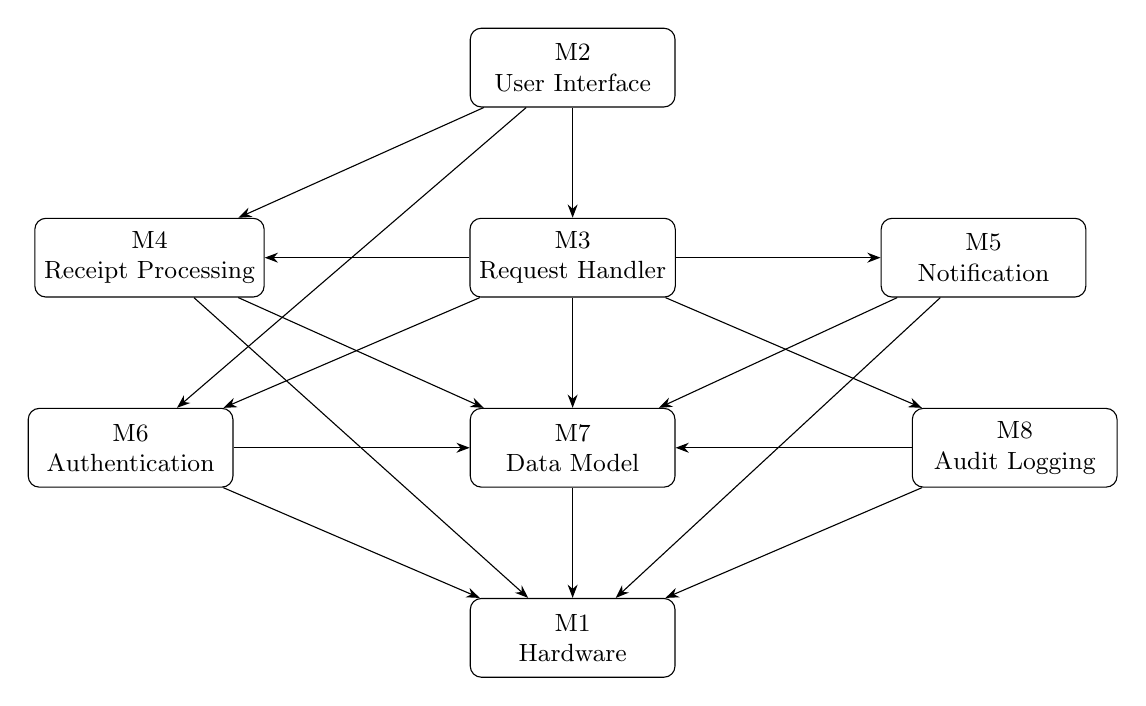
\begin{tikzpicture}[node distance=1.6cm and 2.0cm, every node/.style={draw, rectangle, rounded corners, align=center, minimum width=2.6cm, minimum height=1cm, font=\small}, >=Stealth]
\node (m1) {M1\\Hardware};
\node[above=1.4cm of m1] (m7) {M7\\Data Model};
\node[right=3.0cm of m7] (m8) {M8\\Audit Logging};
\node[left=3.0cm of m7] (m6) {M6\\Authentication};
\node[above=1.4cm of m7] (m3) {M3\\Request Handler};
\node[left=2.6cm of m3] (m4) {M4\\Receipt Processing};
\node[right=2.6cm of m3] (m5) {M5\\Notification};
\node[above=1.4cm of m3] (m2) {M2\\User Interface};

\draw[->] (m2) -- (m3);
\draw[->] (m2) -- (m4);
\draw[->] (m2) -- (m6);

\draw[->] (m3) -- (m4);
\draw[->] (m3) -- (m5);
\draw[->] (m3) -- (m6);
\draw[->] (m3) -- (m7);
\draw[->] (m3) -- (m8);

\draw[->] (m4) -- (m1);
\draw[->] (m4) -- (m7);

\draw[->] (m5) -- (m1);
\draw[->] (m5) -- (m7);

\draw[->] (m6) -- (m1);
\draw[->] (m6) -- (m7);

\draw[->] (m7) -- (m1);

\draw[->] (m8) -- (m1);
\draw[->] (m8) -- (m7);
\end{tikzpicture}
\caption{Uses relationships between modules.}
\end{figure}

\begin{description}
\item[\textbf{M2} uses $\{M3, M4, M6\}$:] Screens and flows render request data provided by M3 and push user actions back through its APIs, which keeps \texttt{FRQ-1}--\texttt{FRQ-3} behaviour identical across clients. Upload widgets stream binaries to M4 so that the receipt constraints in \texttt{FRQ-4} and \texttt{SaL-3} are enforced once instead of being re-implemented in the browser. Role-aware rendering and secure navigation rely on session hooks from M6, satisfying \texttt{FRQ-6}, \texttt{APP-3}, and the accessibility targets in \texttt{ABL}.
\item[\textbf{M3} uses $\{M4, M5, M6, M7, M8\}$:] Request lifecycle logic calls M6 first to confirm the actor's role (\texttt{FRQ-6}, \texttt{SAF-1}), persists changes through M7 to preserve transactional integrity and the latency/capacity bounds in \texttt{SaL-1} and \texttt{CAP-1}, and records each transition via M8 (\texttt{FRQ-5}, \texttt{AUD-1}, \texttt{AUD-2}). When payloads contain receipts, M3 streams to M4 to reuse validation and OCR logic mandated by \texttt{FRQ-4}. Workflow outcomes emit events to M5 so stakeholders receive acknowledgements and escalations without embedding channel logic in the handler.
\item[\textbf{M4} uses $\{M1, M7\}$:] The receipt pipeline calls storage, OCR, and queueing facilities supplied by M1 (e.g., AWS S3/Textract) to meet \texttt{SaL-3} while remaining replaceable. Metadata for every file, checksum, and extraction result is persisted through M7 so that receipts remain linked to their originating requests (\texttt{FRQ-4}, \texttt{PRI-1}).
\item[\textbf{M5} uses $\{M1, M7\}$:] Notification templates are rendered with request, user, and club data fetched via M7, ensuring messages reflect the authoritative state described in \texttt{FRQ-2} and \texttt{FRQ-3}. Delivery relies on the email/SMS gateways abstracted by M1, allowing the provider in \acref{acNotification} to change independently while still meeting \texttt{IMM-2} and \texttt{FLT-3} retry expectations.
\item[\textbf{M6} uses $\{M1, M7\}$:] Authentication depends on cryptographic primitives, secrets storage, and SSO adapters from M1 while persisting user profiles, role grants, and refresh tokens through M7. This encapsulation satisfies \texttt{FRQ-6}, \texttt{PRI-2}, and \texttt{INT-2}; higher layers only interact with opaque tokens or guard functions.
\item[\textbf{M7} uses $M1$:] The data model sits directly atop the managed database and backup facilities exposed by M1. By isolating queries, schema migrations, and replication hooks here, the system respects \acref{acDatabase} while insulating \texttt{FRQ-1}--\texttt{FRQ-5}, \texttt{SaL-1}, \texttt{CAP-2}, and \texttt{LNG-2} from upstream change.
\item[\textbf{M8} uses $\{M1, M7\}$:] Audit events are appended to the durable stores defined by M7 and flushed to immutable storage supplied by M1 (e.g., append-only buckets or managed log services). This architecture keeps \texttt{FRQ-5}, \texttt{AUD-1}, \texttt{AUD-2}, and \texttt{SUP-2} compliant without burdening request handlers with vendor-specific retention logic.
\end{description}

\section{User Interfaces}

The user interface will be designed as a responsive web application using Next.js/React with NextUI components and TailwindCSS for styling. Key interface components include:

\begin{itemize}
\item \textbf{Login Portal}: Role-based access with McMaster SSO integration
\item \textbf{Club Member Dashboard}: View budget, submit requests, track status
\item \textbf{Reimbursement Submission Form}: Upload receipts, enter expense details
\item \textbf{Admin Review Panel}: Approve/reject requests, manage clubs/users
\item \textbf{Audit Trail Viewer}: Access logs and financial reports
\end{itemize}

The interface will follow MES branding guidelines and WCAG 2.1 AA accessibility standards.

\section{Design of Communication Protocols}

The system will use the following communication protocols:

\begin{itemize}
\item \textbf{RESTful APIs}: For frontend-backend communication using JSON format
\item \textbf{HTTPS/TLS 1.2+}: For all network communications to ensure security
\item \textbf{WebSockets}: Optional for real-time notifications (future enhancement)
\item \textbf{SMTP/Email API}: For notification delivery to users
\end{itemize}

\section{Timeline}

The development timeline is structured as follows:

\begin{itemize}
\item \textbf{November 2025}: Complete POC
\item \textbf{March 2026}: Basic components completed
\item \textbf{April 2026}: Testing and integation completed
\end{itemize}

Team responsibilities:
\begin{itemize}
\item \textbf{Zhenia Sigayev}: Authentication Module (M6), Audit Logging (M8)
\item \textbf{Justin Ho}: User Interface Module (M2), Styling and Accessibility
\item \textbf{Thomas Wang}: Request Handler Module (M3), Business Logic
\item \textbf{Michael Shi}: Data Model Module (M7), Database Design
\item \textbf{Johnny Qu}: Receipt Processing (M4), Notification Module (M5)
\item \textbf{All}: Integration testing, documentation, and deployment
\end{itemize}

\bibliographystyle {plainnat}
\bibliography{../../../refs/References}

\end{document}
